% !TeX root = ./main.tex

\chapter{系统设计与实现}\label{ch:system}

\section{总体架构}\label{sec:sys-arch}

系统围绕``知识库构建''和``在线问答''两条链路展开，总体架构如图~\ref{fig:architecture} 所示。

\begin{figure}[htbp]
\centering
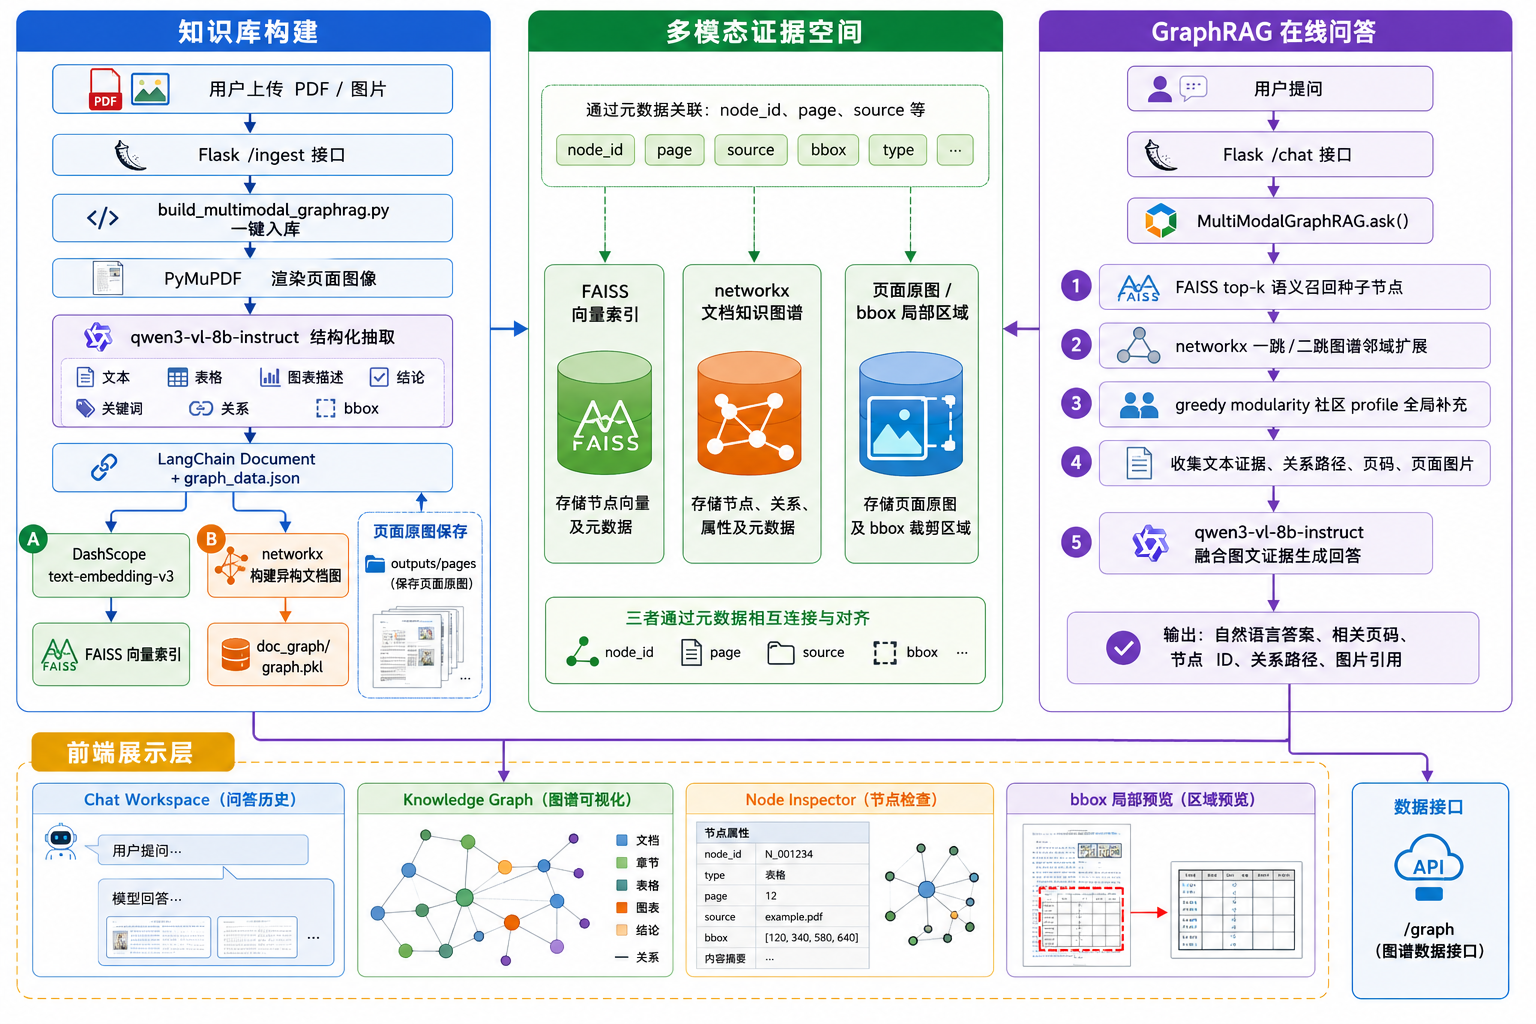
\includegraphics[width=\textwidth,keepaspectratio]{DocRAG架构.png}
\caption{系统总体架构}
\label{fig:architecture}
\end{figure}

\textbf{知识库构建链路}通过 Flask \texttt{/ingest} 接口接收文件后，调用 \texttt{build\_multimodal\_graphrag.py} 执行入库：PyMuPDF 将 PDF 渲染为页面图像，qwen3-vl-8b-instruct 进行结构化抽取得到文本、表格、图表、结论、关键词和关系，封装为 LangChain \texttt{Document} 对象。同一批内容被分别写入 DashScope \texttt{text-embedding-v3} 生成的 FAISS 向量索引和 networkx 异构文档图。FAISS 索引、图谱和页面原图通过 \texttt{node\_id}、\texttt{page}、\texttt{source}、\texttt{bbox} 等元数据对齐，形成统一的多模态证据空间。

\textbf{在线问答链路}从 \texttt{/chat} 接口进入 \texttt{MultiModalGraphRAG.ask()}：FAISS 语义召回种子节点 → 图谱邻域扩展与二跳桥接 → 社区 profile 全局补充 → 融合文本证据、关系路径与页面原图为多模态 prompt → VLM 生成可追溯答案。前端提供 Chat Workspace、vis-network 图谱可视化和 Node Inspector 三个核心交互区域。

\section{文档解析与结构化抽取}\label{sec:sys-parsing}

系统使用 PyMuPDF 将 PDF 页面以 2.0 倍缩放渲染为 PNG，调用 qwen3-vl-8b-instruct 进行七字段结构化抽取：\texttt{texts}（正文/标题/图注，含 bbox）、\texttt{tables}（Markdown 表格）、\texttt{figures}（图表编号/描述/bbox）、\texttt{section\_conclusions}（页面结论）、\texttt{entities}（命名实体）、\texttt{keywords}（方法/模型/指标等关键词）、\texttt{relations}（三元组语义关系）。

解析模块包含三类鲁棒性策略：抽取稀疏时自动使用高召回 repair prompt 重试；仍缺少文本块时调用 text-only prompt 兜底；JSON 解析使用字符串扫描定位对象边界配合 \texttt{raw\_decode} 容错，非法 JSON 时包装为最小化 text-only Document。所有片段被赋予稳定的 \texttt{node\_id}（基于文档哈希、页码和类型），保留完整元数据用于检索、引用和可视化。

\section{知识图谱构建}\label{sec:sys-graph}

本系统的图谱是面向文档问答定制设计的\textbf{异构文档图}。节点类型包括：内容节点（text、table、figure、conclusion、cross\_page\_text）和关键词节点（以 method/model/dataset/metric/task 等分类前缀组织）。边类型包括：same\_page（同页上下文）、keyword\_hit（关键词与内容锚定）、cooccurrence（同页关键词共现）、continuation（相邻页文本延续）、cross\_page\_merge（跨页合并联系）和 VLM 抽取的语义关系边。

这种设计使图谱不仅能支撑多跳推理，还能捕获版面结构、跨页延续和图表-文本对应关系。系统故意弱化不稳定的实体节点，优先使用关键词和内容锚点作为图骨架。图谱构建后使用 greedy modularity communities 算法进行社区检测，每个社区被表征为包含关键词分布、页面范围和节点统计的轻量 profile，用于问答阶段的全局上下文补充。

\section{向量索引与 GraphRAG 检索}\label{sec:sys-rag}

\subsection{向量索引}

系统通过 LangChain FAISS 集成和 DashScope \texttt{text-embedding-v3} 构建本地向量索引（支持切换本地 HuggingFace 模型）。每个 Document 的 \texttt{page\_content} 在嵌入前拼接类型标签和页码信息以增强类型感知。FAISS 索引支持增量更新：通过 SHA-256 文件签名检查文档是否已存在于 \texttt{build\_meta.json} 注册表，仅对新文档执行解析和嵌入。

\subsection{多阶段检索与生成}

问答链 \texttt{MultiModalGraphRAG} 的检索过程分三阶段：（1）FAISS top-k（默认 k=3）语义召回种子节点，支持 \texttt{source\_hint} 限定文档源；（2）在文档图中从种子节点执行一跳邻域扩展（same\_page、keyword\_hit 等），再通过关键词 hub 做二跳桥接，总节点上限 18；（3）将查询词与社区 profile 匹配，按命中数、重叠度和规模选择全局补充证据。

检索完成后构造五层多模态 prompt：任务指令 → 图谱关系链 → 全局社区证据 → 文本证据块 → 相关页面原图（base64 data URI）。最终由 qwen3-vl-8b-instruct 生成答案，返回 \texttt{GraphRAGResult}（含答案、页码、节点 ID、关系路径、图像路径）。系统通过 \texttt{use\_vectorstore}、\texttt{use\_graph}、\texttt{use\_images} 三个布尔标志支持五种消融模式（full/vector\_only/graph\_only/no\_image/none）。

\section{后端与前端}\label{sec:sys-web}

后端基于 Flask 提供 RESTful API：\texttt{/ingest}（文件上传入库，支持 token 鉴权和互斥锁防并发）、\texttt{/chat}（问答，返回答案与引用）、\texttt{/graph}（图谱 JSON，gzip 压缩、含节点级元数据）、\texttt{/node/<id>}（节点懒加载）和 \texttt{/outputs/<path>}（静态文件访问）。工程优化包括：图谱 mtime 缓存自动失效、大响应 gzip 压缩和文件名安全清洗。

前端为单页应用（\texttt{web/index.html} + \texttt{web/app.js}），核心功能包括：Chat Workspace（Markdown 答案渲染、多轮对话）、Knowledge Graph（vis-network 交互式图谱，禁用物理引擎处理 6000+ 节点场景）和 Node Inspector（节点详情、页面预览和 bbox Canvas 裁剪展示）。
